\documentclass[tikz,border=9pt]{standalone}
\usepackage{amsmath,amssymb}
\usetikzlibrary{arrows.meta,positioning,calc}
\definecolor{ink}{HTML}{24364B}
\definecolor{source}{HTML}{EAF1F8}
\definecolor{target}{HTML}{E9F5F0}
\definecolor{accent}{HTML}{257A69}
\begin{document}
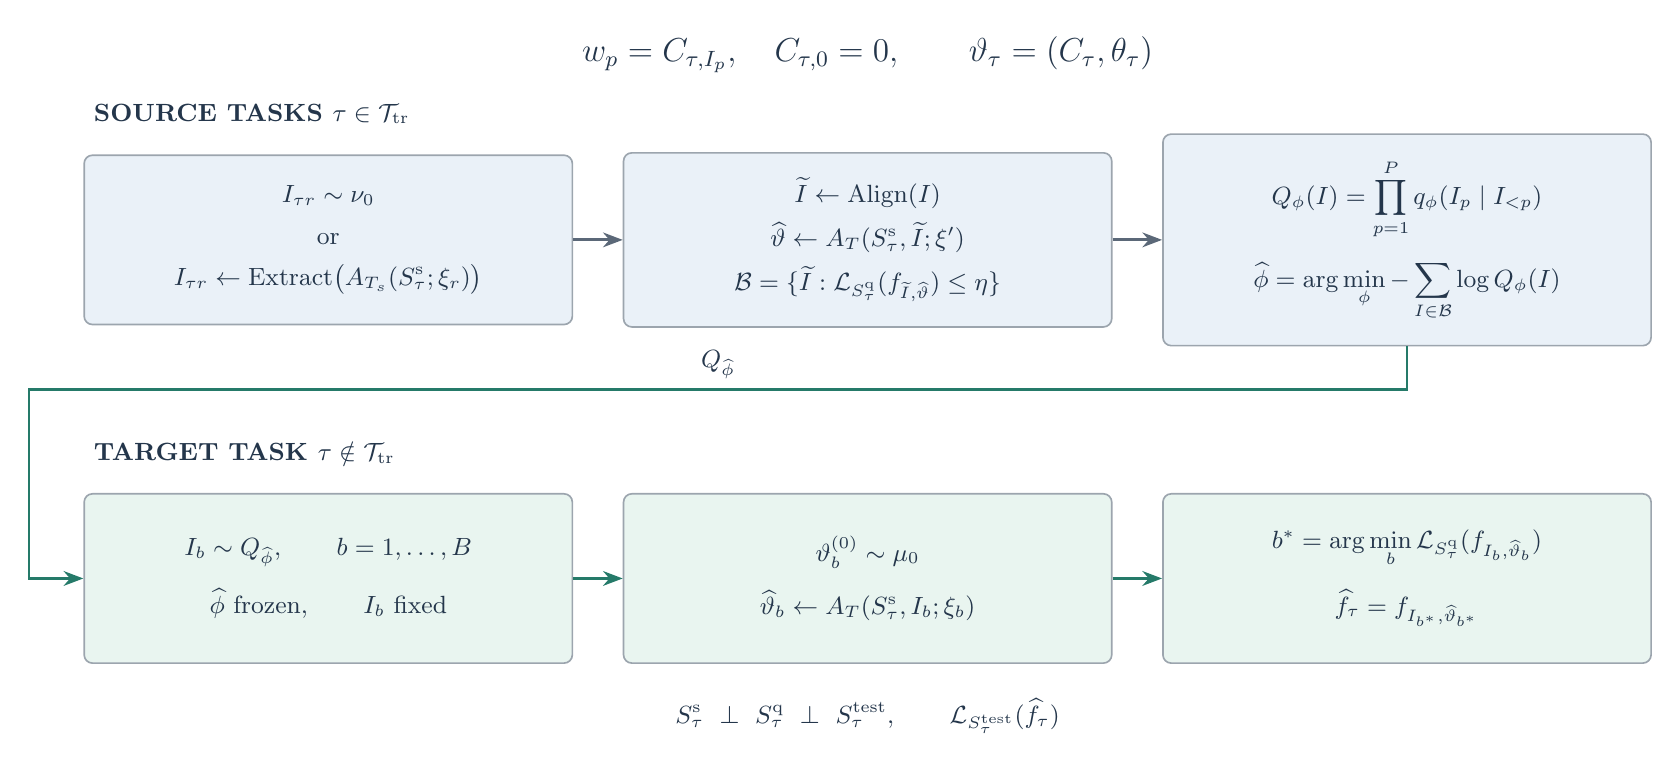
\begin{tikzpicture}[
    font=\small, text=ink, >={Stealth[length=2.5mm]},
    box/.style={draw=ink!45, rounded corners=3pt, line width=.6pt,
        minimum width=6.2cm, minimum height=2.15cm, align=center,
        inner sep=9pt},
    flow/.style={->,line width=1pt,draw=ink!75}
]
\node[font=\large] at (6.85,2.35)
    {$w_p=C_{\tau,I_p},\quad C_{\tau,0}=0,\qquad
      \vartheta_\tau=(C_\tau,\theta_\tau)$};
\node[anchor=west,font=\bfseries\small] at (-3.1,1.6)
    {SOURCE TASKS $\tau\in\mathcal T_{\mathrm{tr}}$};
\node[box,fill=source] (solutions) at (0,0) {
    $I_{\tau r}\sim\nu_0$\\[4pt]
    $\text{or}$\\[4pt]
    $I_{\tau r}\leftarrow\operatorname{Extract}
      \bigl(A_{T_s}(S_\tau^{\mathrm s};\xi_r)\bigr)$};
\node[box,fill=source] (bank) at (6.85,0) {
    $\widetilde I\leftarrow\operatorname{Align}(I)$\\[4pt]
    $\widehat\vartheta\leftarrow
      A_T(S_\tau^{\mathrm s},\widetilde I;\xi')$\\[4pt]
    $\mathcal B=\{\widetilde I:
      \mathcal L_{S_\tau^{\mathrm q}}
      (f_{\widetilde I,\widehat\vartheta})\leq\eta\}$};
\node[box,fill=source] (prior) at (13.7,0) {
    $Q_\phi(I)=\displaystyle\prod_{p=1}^{P}
      q_\phi(I_p\mid I_{<p})$\\[7pt]
    $\widehat\phi=\displaystyle\arg\min_\phi
      -\sum_{I\in\mathcal B}\log Q_\phi(I)$};
\draw[flow] (solutions) -- (bank);
\draw[flow] (bank) -- (prior);
\node[anchor=west,font=\bfseries\small] at (-3.1,-2.7)
    {TARGET TASK $\tau\notin\mathcal T_{\mathrm{tr}}$};
\node[box,fill=target] (sample) at (0,-4.3) {
    $I_b\sim Q_{\widehat\phi},\qquad b=1,\ldots,B$\\[7pt]
    $\widehat\phi\ \text{frozen},\qquad I_b\ \text{fixed}$};
\node[box,fill=target] (fit) at (6.85,-4.3) {
    $\vartheta_b^{(0)}\sim\mu_0$\\[7pt]
    $\widehat\vartheta_b\leftarrow
      A_T(S_\tau^{\mathrm s},I_b;\xi_b)$};
\node[box,fill=target] (select) at (13.7,-4.3) {
    $b^*=\displaystyle\arg\min_b
      \mathcal L_{S_\tau^{\mathrm q}}
      (f_{I_b,\widehat\vartheta_b})$\\[7pt]
    $\widehat f_\tau=f_{I_{b^*},\widehat\vartheta_{b^*}}$};
\draw[flow,draw=accent] (sample) -- (fit);
\draw[flow,draw=accent] (fit) -- (select);
\draw[flow,draw=accent] (prior.south) -- (13.7,-1.9)
    -- node[above,font=\small] {$Q_{\widehat\phi}$} (-3.8,-1.9)
    -- (-3.8,-4.3) -- (sample.west);
\node[font=\small] at (6.85,-6.05)
    {$S_\tau^{\mathrm s}\ \perp\ S_\tau^{\mathrm q}
      \ \perp\ S_\tau^{\mathrm{test}},\qquad
      \mathcal L_{S_\tau^{\mathrm{test}}}(\widehat f_\tau)$};
\end{tikzpicture}
\end{document}
